\documentclass[a4paper]{article}

%%%%%%%% CREATE DOCUMENT STRUCTURE %%%%%%%%
%% Language and font encodings
\usepackage[english]{babel}
\usepackage[utf8x]{inputenc}
\usepackage[T1]{fontenc}
%\usepackage{subfig}

%% Sets page size and margins
\usepackage[a4paper,top=3cm,bottom=2cm,left=2cm,right=2cm,marginparwidth=1.75cm]{geometry}

%% Useful packages
\usepackage{tabularx}
\usepackage{amsmath}
\usepackage{amssymb}
\usepackage{graphicx}
%\usepackage[colorlinks=true, allcolors=blue]{hyperref}
\usepackage{caption}
\usepackage{subcaption}
\usepackage{sectsty}
\usepackage{apacite}
\usepackage[authoryear, round]{natbib}
\usepackage{float}
\usepackage{titling} 
\usepackage{blindtext}
%\usepackage[square,sort,comma,numbers]{natbib}
\usepackage[colorinlistoftodos]{todonotes}
\usepackage{xcolor}
\definecolor{darkgreen}{rgb}{0.0, 0.4, 0.0}



%%%%%%%% DOCUMENT %%%%%%%%
\begin{document}

%%%% Title Page
\begin{titlepage}

\newcommand{\HRule}{\rule{\linewidth}{0.5mm}} 							% horizontal line and its thickness
\center 
 
% University
%\textsc{\LARGE Goettingen University}\\[1cm]

% Document info
%\textsc{\Large Masters Economics}\\[0.2cm]
%\textsc{\large Urban Economics}\\[1cm] 										% Course Code
\HRule \\[0.8cm]
{ \huge \bfseries How DRT Systems Can Protect Overburdened Traffic Systems from Congestion Collapse}\\[0.7cm]								% Assignment
\HRule \\[2cm]
\large
											% Author info
{\large \today}\\[5cm]
%\includegraphics[width=0.6\textwidth]{images/BGU.sig3-he-en-white.png}\\[1cm] 	% University logo
\vfill 
\end{titlepage}

\begin{abstract}

This article addresses issues of transport system design through simulation of  demand responsive transport systems and its impact on relieving  congestion in the context of a developing city, Cape Town, South Africa. Cape Town is struggling with high levels of congestion, which we hypothesize can be addressed through demand responsive transport as an emerging technology. The results of our simulation study, which introduces demand responsive transport options, shows a reduction in congestion, whilst otherwise also providing a socially desirable solution. The findings can be harnessed in other settings like Cape Town for pushing forward transport system design for economic and social improvement. Furthermore, the usefulness of simulation with an Agent-Based model such as MATsim proves to provide a useful application for research and policy advice.


\end{abstract}

%%%% SECTIONS
%% Section 1
\section*{Introduction}

Large scale urbanisation has accompanied the huge economic growth the world has seen since the industrial revolution \citep{ritchie2018urbanization}. This trend continues with the developing world now having the highest urbanisation rates. Concurrently with urbanisation, the revolution of modern transport has shaped life as we know it today \citep{rodrigue2020geography}. The story of the 'American Dream' and Ford advertising for every American family to have an “automobile” has translated into reality across the world, Africa being no exception. Car imports into Africa have been rising with the growing African middle class driving demand \citep{organisation2018africa}. These factors are causing increasing traffic congestion pressure in cities. Inefficient transport systems have negative externalities in many sectors of the economy \citep{jabbarpour2018applications, miskolczi2021urban}. As such mobility has become a policy issue high on the political agenda in most cities \citep{costa2017urban, miskolczi2021urban, perveen2017evaluating}. This is further exacerbated by underinvestments in road infrastructure and public transport in many developing nations. Congestion in turn affects emissions and negatively externalities such as reducing social wellbeing and can reach levels that are detrimental to urban development. It has for example been noted that premature deindustrialization is a problem countries in Africa and Latin America face \citep{mcmillan2011globalization}. 
Thus the costs of congestion can spillover beyond individuals to city-wide stagnation and hinder national development. 

A functioning and productive economy requires the efficient movement of people and goods. Traffic congestion, caused by excessive levels of travel demand by private cars, has large opportunity costs such as increased transaction costs and productive hours spent driving. In addition, freight movement impacts supply chains whilst local businesses bear costs with sluggish movement of goods or services that require physical movement. Thus dealing with traffic congestion in various ways including the management of travel demand, is necessary for economic efficiency. 
%From a sustainability point of view there is also a great need to reduce the number of non-electric cars on the road \citep{miskolczi2021urban}.

Solutions to reduce congestion are varied, and whilst trying to maintain levels of accessibility in the city, systems thinking can improve the way this complex issue is approached. More optimal outcomes can be reached for the goals of city development and welfare within the constraints of population and infrastructure with certain advanced modelling techniques \citep{ccolak2016understanding}. Agent Based Modelling (ABM) scenarios, for example, can be constructed to experiment and compare accurate outcomes for policies to eventually improve transport outcomes in cities. 

One useful transport design innovation that can help cities address congestion is Demand Responsive Transport, which is a technology-enabled shared mobility service. Demand Responsive Transport (DRT) is seen  as a helpful addition to developed country transport systems across the world \citep{Ben-dor, engelhardt2019quantifying, schluter2021impact, kaddoura2020impact,maggi2021price, miskolczi2021urban, zwick2021ride, article}. New technology, growing urbanisation and pressing environmental and efficiency needs to reduce private cars, have led to efforts to design optimal transport around users \citep{ronald2015simulating}. DRT design and simulation is a burgeoning field of research with the potential to bring disruptive technologies to solve urgent social and environmental problems \citep{schluter2021impact}. This emerging transport technological  innovation needs further exploration in a developing country context. Our paper studies the potential effects of introducing several DRT implementation scenarios in Cape Town, South Africa, using an Agent-Based simulation platform, MATsim. The scenarios we study include varying fleet sizes between 1000 - 3000 vehicles in the city, with fares ranging between double and triple the public transport price, and DRT design either being stop based or a door to door service. We hypothesize that DRT has the potential to significantly reduce congestion, because of a decrease in private car use and traffic flow optimisation, and we simulate different scenarios for optimal effects. The article is structured with a literature review in the next section, after which we present a methods section. A results section follows and finally the conclusion and further research is laid out. \\



% Finding alternatives and exploring the reshaping of urban transport systems is necessary. DRT is one such alternative of a transport mode that could improve transport system’s efficiency and outcomes. However, little is known about the system wide effects that introducing such an intervention would bring, especially in developing country cities such as Cape Town. Simulation allows for the evaluation of scenarios of DRT without the costs of implementation and can help with optimal design to reduce congestion and emissions. This study carries out a simulation of the introduction of a new alternative DRT in Cape Town and evaluates the output for its effect on congestion for different areas of the city and emissions.

\section*{Literature Review}
\subsection*{Demand Responsive Transport}

DRT has been around since the 1970's - 1990's with several variations in the meaning of the term itself, but its use has increased and reached greater clarity and consensus since the early 2000's.
The basic idea of DRT is that of transport that is provided flexibly in response to signals for demand by users. \citealp{butler2020smart} define DRT as being able to change route and or schedule depending on demand. DRT has been classified into several forms, and it overlaps with the categories of paratransport and shared mobility  \citep{butler2020smart}.
It can either be area-based or line-based, with door to door random stops or set stop points when it is stop based. It can be ad-hoc such as minibus taxis (MBT's) in South Africa or real-time centrally coordinated such as MOIA in Hamburg, Germany. Sometimes DRT has been referred to with terms such as ride hailing, ride sharing, demand responsive transit or flexible transit services. \citealp{vansteenwegen2022survey} investigate demand response public bus systems. Within their framework they undertake  a many-to-many fully flexible door to door design, with some stop based scenarios for the  DRT modelling. For many-to-many fully flexible design, there can be many pick up points which drop at many drop off points and the route can be adjusted while in transit according to new pickups.
Real-time centrally coordinated DRT has clear advantages to gain by using app based technology for dynamic requests and routing \citep{zwick2021ride}. In this paper DRT refers to real-time centrally coordinated DRT. Emerging technology allows the scale and efficiency of a DRT system to be a powerful opportunity to harness in cities with the need of increased efficiency of transport options. Many companies have joined in the surge to introduce attractive DRT options across the world \citep{zwick2021ride}.  MOIA, BART, Telebus, Omnilink (Virginia), dial-a-ride transit (DART), scheme in Winnipeg, Manitoba, are all examples of existing DRT companies in developed countries. Fleet size of existing services ranges from 50 to 6000 \citep{zwick2021ride}.
DRT that carries more than one passenger from more than one pick up point has the potential to decrease the number of vehicles on the road when users that used to drive separate cars now pool their trips \citep{zwick2021ride}. The key to sharing is a higher utilization of goods by replacing permanent individual ownership by temporary on demand access \citep{botsman2010s}.
Some have classified DRT under car sharing in the business to consumer category \citep{munzel2018carsharing}, while others categorise DRT separately from car sharing and shared mobility \citep{butler2020smart}. Whether it is classified together with sharing or not, the bottom line is that DRT vehicles service many more users than a private car would. And it would give greater sustainability improvement for electric and autonomous vehicles. The general need to improve transport in cities has been termed ‘smart urban mobility’\citep{butler2020smart}. DRT is one method among many innovative solutions geared towards sustainability \citep{butler2020smart}. \\

A literature survey on urban mobility scenarios by \citealp{miskolczi2021urban} found four main research perspectives with alternative forecasts, and conclude that the most likely outcome is a slow shift to emerging technologies of ride sharing, electric and self-driving vehicles.
Travel time is important in decisions to use transport modes such as DRT \citep{reck2020shared}, and high fares do not necessarily deter use of public transport \citep{tyrinopoulos2013factors}. Thus prioritising efficient transport for lower congestion and time costs is a good priority to have, and aligns well with the expectation of the literature of a shift to increasing use of DRT and similar emerging technologies. DRT allows for the use of emerging technologies to optimise flow of traffic and decrease vehicles per person on the road. 
%distance, design of city, land use, road network, public transport, incentives such as tolls.\\
Congestion is a complex phenomenon \citep{arnott1994economics}.
\citealp{butler2020smart} note the effects of DRT on congestion can be both positive and negative, because although cars per passenger decreases and traffic flow increases because of adaptive planning, pick up and drop off zones can increase congestion, and vehicle numbers can increase with higher accessibility or preference for low occupancy vehicles. These issues must be monitored with pilots after simulation. Furthermore, land use and urban planning must coincide with purely mobility focused solutions to obtain the most efficiency \citep{jabbarpour2018applications}.\\

Small decreases in  travel demand can have large impacts on solving congestion, and improving travel time \citep{vickrey1969congestion}.
This however, requires particular conditions, as congestion is often not only becuase of physical bottlenecks \citep{arnott1994economics}. Using Agent Based Modelling the modeller is able to deal well with complexity and individual decisions which gives confidence to the predicted change in congestion we investigate. Findings have shown that scenarios with automated DRT taxis in Berlin could eradicate congestion in the city if road capacity increases continue at the projected rates \citep{maciejewski2016congestion}.\\


%\subsection*{Simulation}


Literature on Demand Responsive Transport simulation has been investigated by \citealp{ronald2015simulating}, and they highlight Agent Based Modelling (ABM) to be an useful tool to simulate DRT before implementing it. ABM uses network theory and focuses on individuals in a system which allows for interaction between operators and users \citep{ronald2015simulating}. MATsim is an open source software that allows traffic system modelling and is based on the concept of ABM.
MATsim simulations have been used in several cities to help plan and design DRT. A simulation for Berlin suggested that low prices and a small service area would lead to unwanted switching from walking and cycling to DRT for short distances \citep{kaddoura2020impact}. When a minimum fee was used to disincentivise the undesirable shift it was found that introducing DRT gave positive effects to transport in the city with lower travel times and higher utility \citep{kaddoura2020impact}.\\

\citealp{schluter2021impact} carried out an impact evaluation on the use of DRT in Bremerhaven, Germany, to connect rural and urban areas. They found that without using automated vehicles DRT could not compete with private vehicle use in Bremerhaven. As private car ownership is much lower in South Africa than in Germany for example, and because the paratransit systems with MBT’s  exemplifies a starkly different transport system in South Africa a case for upmarket and technology enhanced DRT is seen as a worthy alternative to be considered.
\citealp{article} examined a rural DRT case in the town of Colditz in Germany using MATsim, and they found that line-based services would be better than fully flexible services. However this was specific to the rural case where population and demand density is low. In urban cases like Cape town, population and demand density in areas that feed the CBD should be much higher.
DRT for automated vehicles has also been modelled with an example of \citealp{Ben-dor} who found that the optimal fleet size for Tel Aviv to have its transport needs covered by this form of transport was 50 000 to 150 000. \citealp{medina2019public} find a novel way to model DRT in MATsim and apply it to a new suburb to be developed in Singapore.
\citealp{engelhardt2019quantifying} also use MATsim for simulating ride pooling efficiency in Munich Metropolitan Region and find that the greater the density of trips the more efficient ridepooling is.\\
The mobiTopp simulation of MOIA in Hamburg performs an evaluation of a DRT system in Hamburg with varying fleet number, areas covered and autonomous vehicles \citep{MOIA}. They find that the increasing the use of DRT has a positive effect on the use of public transport instead of 'cannibalising' it, which is often a hypothetical argument against introducing DRT. Furthermore in their research the large fleets with autonomous vehicles lead to the lowest costs \citep{MOIA}.\\
The number of cities with MATsim modelling frameworks and applications has been increasing across the world and includes Berlin, Sao Paolo, Lille Metropolis, San Tiago, Zurich, Basel, Vienna, Lagos, Casablanca, Cape Town and the San Francisco bay area \citep{kaddoura2020impact, sallard2020agent, kickhofer2016creating, balac2021synthetic, diallo2021agent, ilahi2019existing, kagho2019agent, becker2018matsim, muller2021matsim, benhlima2021towards}.
\\

%\subsection*{Related issues}

A closely related theme of research to DRT is Mobility-as-a-service (MaaS). The idea behind MaaS is to have integrated transport offerings within city or regional systems \citealp{Loubser}. DRT is often seen as playing a key role in MaaS. 
MaaS in Zurich, Switzerland, for example, is modelled using MATsim and found to give higher efficiency and lower emissions \citep{becker2020assessing}.
Initial modelling of DRT in Cape Town could pave the way for DRT in a MaaS framework.
MaaS in the context of developing countries  has received little attention. 
\citealp{Loubser} cite the potential for on demand shared transport and MaaS paratransit efficiency. Part of the broader research advocated by the \citealp{Loubser} is an introduction of technology into the paratransport system that could compliment insufficient public transport, and be part of a larger system. The low penetration of smartphones in poorer areas restrict app requirements to more affluent communities in developing countries. The MBT's in developing countries, although demand responsive, lack the efficiency and extreme flexibility of a many-to-many algorithm controlled DRT system that could be introduced. \citealp{vanderschuren2018ride} look into ridesharing possibilities in developing contexts using survey data. Their findings are that there is a high likelihood of DRT most likely being mostly used for shopping and services rather than for work and education trips. 
In a different context \citealp{yu2019exploring} use on-demand ride sharing data from Washington to explore spatial variation and built environment impacts on demand for ride sharing. Their findings show that weekday and weekend demand changes for different income categories of the population \citep{yu2019exploring}. Further an important finding they have is that mixed land use has a very large impact on the demand for ride sharing services. This can point to considering landuse in areas where DRT is offered. It also leads to suggestions for land use planners to encourage mixed land use for integration with transport systems that facilitate accessibility.
\citealp{maggi2021price} found motivation-based policies were more effective than price based in motivating switches to environmentally better transport modes, and that a soft mix between the two was best. 
As our simulation would primarily have time and price based switching, it can be interpreted as a lower bound of modal switching without preference influencing policy or marketing being implemented to increase the switching.
\citealp{maggi2021price} used ABM on Italian data. They point out the weaknesses of ABM; that it requires accurate parameters and it suffers the same tension as all models of parsimony and realism. \\



%Cape Town: accessibility, MBT, BRT (history),areas and design, uber, golden arrow. \\

\subsection*{Transport in Cape Town}

Cape Town is the second largest city in South Africa and it is one of the most advanced cities of Africa. However, it is commonly criticised for its underdeveloped public transport system (in particular rail) that uses high levels of household incomes, long walking distances and waiting times and congestion \citep{StateofCT, jennings2015finding}.
Congestion frustrates drivers with high fuel costs and travel times. Those who use public transport often have long queues, over-crowding and delays \citep{jennings2015finding}.
Cape Town city design is such that it is a “low density city” with urban sprawl that places most residents on the periphery \citep{Turok2011, jennings2015finding}. Transport occurs in tidal form and public transport trips are mainly to and from the centre \citep{Turok2011, jennings2015finding}. Public transport waiting times are high and travel times are generally high in the city. \citealp{hitge2015comparison}, note the difference in travel time of public transport versus private transport in Cape Town. DRT in a context like this would give a potentially faster option to bridge the time and price gap between public and private transport options in Cape Town. They also reason for accessibility \citep{hitge2015comparison}.
%"The average travel time in Cape Town was, at about 90 minutes in 2013, at the upper end of the global range, which averages around 70 minutes per person perday (Metz 2010; Schafer & Victor 1998)."
The Statistics South Africa transport survey Western Province report, reveals that many Cape Town residents (14.8 percent) cite congestion as the main traffic problem experienced  \citep{StatsSAreport}.
12 and 11.2 percent respectively record that non-availability of buses in their area and reckless taxi drivers are their main concerns \citep{StatsSAreport}. 
Travel time was the most common determinant of transport mode choice (32.5 percent) in the 2013 National Household Travel Survey \citep{StatsSA14}.
These community survey results give evidence that the experience of city residents points to problems of congestion and lack of public transport options that DRT could contribute to solutions for these problems experienced. \\

Rail provision in Cape Town faces many challenges as cited to have “overcrowding, slow journey times, poor modal integration, a lack of off-peak services, manual ticketing and an irregular timetable” \citep{TDCIP}. Congestion is also seen as a rising problem in the city \citep{TDCIP}. The problem of congestion is recognised by the transport authorities as costly on time, money and environmental impacts, and they have developed a “Congestion Management Plan”. This plan would incorporate operational, behavioural and infrastructure components and DRT could be a helpful addition for consideration in this plan.
Congestion inhibits accessibility for all who use roads to reach their destinations. As time is a valuable resource and the poor have greater opportunity cost as a risk to livelihood and share of income, there is great impetus to decrease congestion for the sake of poor road users. \citealp{jennings2015finding} notes the long travel times experienced in Cape Town, and the problem of congestion experienced as traffic converges from surrounding areas on the CBD. 2013 data showed that travel took 71 percent longer than it would without congestion - these are large costs for a city to bear \citep{TDA}. The economic costs have been estimated by some in 2018 to be 2.8 billion rand \citep{IOL}. 2022 infrastructure projects to deal with congestion cost 192 million rand and the total for capacity improvement and running transport in the city is 6.4 billion rand over 3 years \citep{TCT}. These spending items reveal the city's estimations of the cost of congestion that they can address with their budget and the importance of efficient transport to the city.\\
%Cape Town has been experiencing high levels of congestion in the last 20 years, and in 2015 a summit was held on congestion and policy was put in place to manage congestion. Since 2006 conscious measures of behavioural influence have been on the city agenda. The problem however has remained one that requires constant attention, as in many other cities.


Accessibility has been raised as a key framework for transport design and justice \citep{Access}. It is especially important in Cape Town which has a history of discriminatory exclusionary policy that impacted city design and thus transport corridors. Unemployment and spatial segregation in the city form an exclusionary combination that need addressing with better transport and landuse planning. Introducing DRT into richer areas of the city can pave the way for increased accessibility in these areas for job seekers, and the profitable areas can lead to a pilot for the government to consider subsidising similar systems in other areas to complement or replace their subsidy of transit buses currently. \citealp{Moyo} found that middle income areas have more mixed land use, while poor areas remain homogenous. Combining this with knowledge on the higher uptake of DRT in mixed landuse scenarios it would make sense to first investigate the more affluent areas of Cape Town for DRT viability \citep{yu2019exploring}.
Design of DRT could be incorporated or complement future transit system redesign \citep{byala2021redesigning}.
Cape Town City is aiming to increase road capacity and public transport for low income areas in the next five years \citep{IDP}. The problem of congestion will likely still exist even with these interventions and DRT could be a useful complement to these efforts, especially as they do not focus on affluent areas which contribute large amounts of vehicles. \citealp{byala2021redesigning} note that new mobility such as DRT can be incorporated into redesigning bus systems, this could be a beneficial exercise in the future of Cape Town’s traffic design as the city changes and grows and demand for transport and its efficiency increases.\\

The International Network for Transport and Accessibility in Low Income Communities (INTALInC) report "Transport and social exclusion in five African cities June 2019" gave suggestions of the need for local scenario studies and comparative studies \citep{lucas2019transport}. Simulations with locally calibrated data fills this gap and harnesses the power of big data to help understand and solve social problems.
\citealp{vanderschuren2018ride} evaluate the potential market for ridesharing in Cape Town using the 2013 national transport survey data. Their research is constrained by lack of quantitative data and relies on expert opinion. 
Using agent based modelling to simulate the city transport system fills this gap of lacking data, and we can investigate their conclusions that low income households would switch to ridesharing solutions and DRT could have an important role to play in filling the transport demand in the city.
There are many studies on DRT simulations and outcomes, but none that focus on congestion in developing contexts. This study attempts to fill this research gap.\\

\section*{Method}

% research question (suburbs) and scenarios 
This paper investigates the effect on congestion from introducing DRT to affluent suburbs surrounding three of Cape Town's key economic hubs (CBD, Kenilworth and Bellville). These areas have higher potential to afford more expensive transport options than the low quality public transport services, and these areas also receive less prioritisation for public transport funding and therefore market solutions can solve the lack of public infrastructure \citep{TDCIP}. Figure \ref{fig:1} shows a map of Capetown with different employee anual income quintiles from census data \cite{Statistics_South_Africa} and our modelled service areas. We model scenarios of varying fleet size, pricing and stop design to evaluate congestion effects. These areas also have high levels of congestion and private car use as they are business centres in the sprawling city. Congestion is a major problem to be tackled, and experimenting and optimising with innovative transport modes such as DRT addresses this issue and can add values to cities as one way to tackle congestion.\textcolor{red}{@Alex wo steht wie das Bediengebiet ausgewählt wurde?} \textcolor{red}{@Jan die wurden nach dem Gespräch mit Justin ausgewählt. Er hat erwähnt, dass die für unsere Analyse relevanten Bevölkerungssschichten außerhalb des CBDs wohnen und aus der oberen Mittelschicht stammen.}\textcolor{green}{@Alex: Dann bitte ergänzen welche Einkommensschichten ausgewählt worden sidn}

%The findings point toward the general effectiveness of introducing DRT for improving congestion in cities, and furthermore that tailored design specification can optimise results. DRT could enter the ranks of transport innovations that revolutionise our world as it decreases congestion that plagues cities around the world, and opens up better mobility for more people.DRT is advantageous as a solution to congestion as it can be implemented incrementally and is much more flexible and adaptable as an investment than large public transport infrastructure. It can complement current transport systems and add value to cities with much needed congestion decreases.

\begin{figure}[!h]
  \centering
    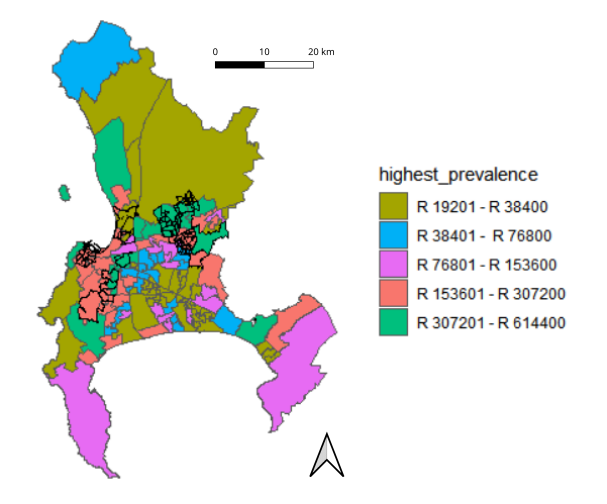
\includegraphics[width=0.65\linewidth]{images/Serv_area_quintile.png}
     \captionsetup{width=.9\textwidth}
     \caption{Highest prevalence household income quintile in Rand per Ward. The map shows that the wards around the defacto CBD's of Capetown are in the higher wealth quintiles which supports our reasoning of better DRT markets in these areas. The Service Areas we model are outlined in black on the map. \citep{Statistics_South_Africa}}
     \label{fig:1}
  \end{figure}


In order to analyze the effects of significant changes to mobility services, we compare the status quo with a hypothetical case that introduces a large fleet of shared demand responsive vehicles that can may be used by Capetown's population. In our study, we take advantage of the multi-agent transport simulation framework MATSim version 14.0 because its highly disaggregated level of analysis allows to investigate the effects of transport policies on travel behavior in the most granular way possible. The upcoming section presents a general overview of MATSim and parameters used in this paper, followed by a description of the Capetown scenario setup and an overview of the shared mobility scenarios applied \citep{Horni.2016}.

\subsection*{MATSim framework and scenario parameters}

MATSim represents travellers in the real world as artificial agents with corresponding socio-demographic attributes and aims to mimic real world travel patterns through an co-evolutionary algorithm. The framework simulates daily activity and mobility patterns of all agents and takes into account mode choice, departure time and route choice.  Movement patterns of road vehicles are simulated on a network graph which represents local infrastructure and carries attributes such as maximum freespeed or road capacity. Interaction between agents on network links with full capacities leads to congestion which is handled in a queue-based first-in-first-out (FIFO) principle \citep{Horni.2016}. 

An integral part of MATSim ability to reproduce real-world mobility patterns is the optimization of agent's behavior through a maximization of an individual score that takes into account the time spent at planned activities and the time and cost spend travelling from one destination to another. In a MATSim simulation, each agent iteratively performs a plan that expresses its preferences in terms of activities, trips and scheduling. Over the course of the iterations, a set of agents modify their plan while others stick to their initial plans. To be able to compare plans with each other, each plan is given a score according to a utility function as described below. The simulation ends after a predefined number of iterations in which an equilibrium is reached in which no agents can improve their score anymore. \\ 

The utility function is formulated as follows: 

 \begin{equation}
S_{\text{plan}}=\sum_{q=0}^{N-1} S_{\text{activity},q} + \sum_{q=0}^{N-1} S_{\text{travel},\text{mode}(q)}
\label{1}
\end{equation}

with

\begin{equation}
\begin{aligned}
   S_{\text{travel},\text{mode}(q)} =   C_{\text{mode}} + \beta_{\text{trav}, \text{mode}(q)} * \text{}_{q} + \beta_{m}*\Delta m_{q} \\
    +\, \gamma_{d,\text{mode}(q)})* d_{\text{travel},q} +\beta_{\text{transfer}} * x_{\text{transfer},q} \\
    +\,  DMC_{\text{mode}} * \lambda_{\text{mode}}
\end{aligned}
\end{equation}
\\ 
Where $q$ equals a leg as part of a trip from origin to destination, $C$ is a mode specific utility constant, $\beta_{\text{trav},\text{mode}}$ the marginal utility of travelling per hour, $\beta_{m}$ is the marginal utility of money that is constant throughout the scenario (1), $\Delta m$ is the money spent on the transport mode, $\gamma_{d,\text{mode}(q)})* d_{\text{travel},q}$ is the monetary distance rate in meters multiplied by the travelled distance and $\beta_{\text{transfer}} * x_{\text{transfer},q}$ resembles a transfer penalty that applies if agents have to switch vehicles within a leg (e.g. in a public transport leg). \citep{Horni.2016}. Additionally, we use a daily monetary fee that is paid by the users each time they use a specific traffic mode ($DMC_{\text{mode}} * \lambda_{\text{mode}}$). This fee can be thought of as car fixed costs or subscription fees for public transport or DRT. Table \ref{Utility values} shows the mode specific utility values for the modes. It becomes evident, that in this setting the travel time using a particular mode does not have a direct effect on the (dis)utility that is obtained by the agent while traveling. However, a strong increase in travel time translates to an agent having less time to increase its utility by performing activities (captured by the first term in equation \ref{1}) and thus having an indirect penalty on a user's score. Thus, agents will avoid being stuck in traffic jam as it increases the overall travel time and thereby decreases their utility score. 

\begin{table}[!h]
\centering
\resizebox{1\textwidth}{!}{%
\begin{tabular}{|l|l|l|l|l|l|}
\hline
Mode             & Constant & Daily monetary constant & Marginal utility of travelling & Monetary distance rate (ct/km) & Transfer utility \\ \hline
Public transport & 0 & -1.9                   & 0                              & 0                             &  -1    \\ \hline
Car              & 0 & -10                     & 0                              & -11                            &  0  \\ \hline
DRT              & 0 & -3.8                    & 0                              & -15                             &  0 \\ \hline
\end{tabular}
}
\caption{Utility values for DRT scenario with double public transport prices}
\label{Utility values}
\end{table}



\subsection*{Capetown scenario and calibration}

A synthetic scenario of Cape Town with a population sample size of 10\,\% is employed for the study. We derive the synthetic population from South African Census Data 2011 \citep{census2011}, the 10\% Public Use Sample \citep{census2011public10pct} and the Minnesota Population Center Integrated Public Use Microdata Series \citep{mpc2020}. For the population synthesis process we employ a mlti-level iterative proportional fitting methodology \citep{joubert2014mipf}. Furthermore, we utilize data from National Household Travel Survey 2013 \citep{nhts2013} and the Time Use Survey 2010 \citep{tus2013} to assign individual mobility behaviour to the synthetic agents. 

On the supply side we employ network and infrastructure data from OpenStreetMap (OSM) \citep{osm}. The network links are downscaled according to the population sample in terms of flow and storage capacities. Furthermore, the individual OSM ids of the dataset are extracted and categorised into different activities such as "shopping" or "leisure". In addition, we use GTFS datasets from the main public transport providers in Cape Town from 2018 to model public transport \citep{transifeeds}. The capacities of the vehicles are also downscaled according to the population sample, as the adjustment of the vehicle size to the downscaled network leads to a distortion of the passenger flows. To avoid further distortions in the timetables of the vehicles by the other network participants and for reasons of simplification, the vehicles of Golden Arrow Bus Services (GABS), Metrorail Western Cape, MyCiTi Cape Town Integrated Rapid Transit (IRT) system and UCT campus shuttle buses (Jammie) operate on a pseudo-network with direct aerial lines between stops and with adjusted speed limits on each route to match the timetable. For the modelling of informal public transport in the form of minibus taxis, the use of a pseudo-network is omitted due to the fact that the number of minibus taxis is significantly higher than in the case of formal public transport which leads to feedback effects in the traffic flow. To represent these effects in the overall traffic in Cape Town the Minibus Taxis travel together with the other individual traffic on the OSM motor roads.\\

Again, using the OSM data, the modelled infrastructure and the socio-demographic characteristics of the agents such as age, gender and employment status, a gravity model is used to create a path-destination matrix and assign it to the agents. The resulting base population then goes through several calibration steps to accurately mimic the real world travel patterns, calibrating towards NHTS averages and Cape Town Vehicle Detection System (VDS) traffic flow data on major roads from 2018. The calibration target is set at an average deviation from real data of less than 20\% error for car traffic and less than 50\% for formal and informal public transport.\\



\subsection*{Shared mobility scenarios and congestion measurement} 
 
The simulation of shared DRT vehicles is performed by the 'dynamic vehicle routing problem' (DVRP) contribution that is available as an extension to MATSim \citep{Maciejewski.2017}. This model allows for an on-line allocation of DRT vehicles, i.e. routing of vehicles dynamically adapts to agents request within the simulation (DRT service cannot be booked in advance). The package allows for variation in fleet size and service type. Several scenarios were explored where fleet size, DRT pricing, and DRT service design are varied. The fleet sizes experimented with and chosen is to optimise as an addition to the existing baseline traffic of Cape Town. The pricing is set at double and triple public transport price because it cannot viably be cheaper than public transport. The pricing factor forms part of the rational behind the choice of service areas, as these high income areas are more likely to be able to afford prices that are higher than public transport, while low income areas already spend high proportions of their income on using public transport. For services types, we (1) adopt a stop-based system that mimics existing public transport station in the network as access/egress station for DRT services and (2) allow for a door-to-door service within the service area. 
 
 The main analysis is on the simulation of a fleet of 300 Door to Door service (DtDs) DRT vehicles at a price twice that of public transport as this was the optimal result for congestion. The model is calibrated to Cape Town traffic and population\footnote{MBT's are included as public transport}. The population have activities of work, education, shopping, leisure and health and various times for their activities which determines their decisions. The simulation is run with 300 iterations. \\


\begin{figure}[h]
\centering
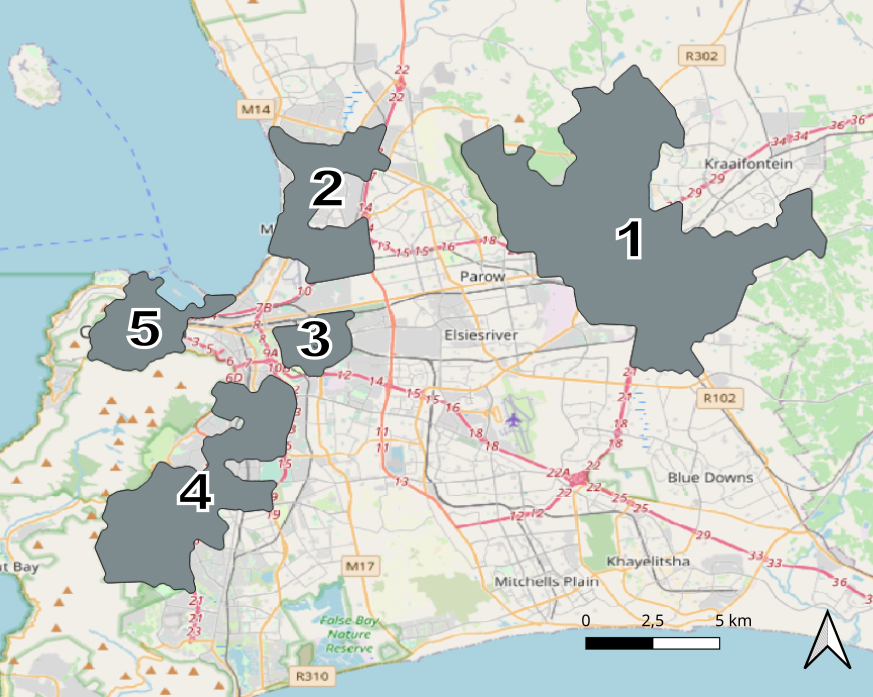
\includegraphics[width=.9\textwidth]{images/serv_area_groups.png}
  \captionsetup{width=.9\textwidth}
  \caption{Connected Service Areas in Capetown for the DRT simulation in grey.}
  \label{fig:7}
\end{figure}

 %\textcolor{red}{Andy to do: Details on the simulation set up are still to be addded. Information will include: data sources used (minibus are part of the simulation), calibration, initial modal split, price sensitivity matsim ...}
 
\section*{Results}

The results from the simulations of various scenarios with 100 and 300 DRT vehicles, which translate to 1000 and 3000 vehicles in the full scale 100 percent situation, show that in all scenarios of adding these small to medium sized DRT fleets, congestion improved in the city. \textcolor{red}{wo sieht man das?}. \textcolor{red}{@Jan Figure 9?}.  This shows hopeful results for adding DRT to transport systems to improve congestion. We analyse the results to understand dynamics and optimal efficiency that can be gained from DRT in the city transport system.\\
\textcolor{red}{@Alex wo kommt 500 her?} \textcolor{red}{@Jan https://doi.org/10.1016/j.procs.2020.03.152 für Berlin nehmen 1k vehicles für 10\% sample für Berlin. Da wir nicht die ganze Stadt betrachten sondern nur einige Gebiete, habe ich einfach vorgeschlagen zu halbieren.}
We found that introducing a fleet of 500 DRT vehicles left many vehicles with empty periods and the scenario wastes the extra vehicles, as the modelled Cape Town transport environment would not induce high enough DRT usage to validate a fleet of 500 without accompanying policy to increase DRT usage. Policy could in theory impact behaviour to induce uptake of DRT, such as in the extreme scenario some have explored where all cars are replaced by DRT \citep{Ben-dor, maciejewski2016congestion}. Alternatively motivation based policies can bring a higher uptake of DRT \citep{maggi2021price}. Furthermore, tolls or other incentive based schemes can impact user transport mode more than merely price and time which is the lower bound organic change which we explore in our modelling. When the fleets of 100 and 300 vehicles at double and triple public transport costs were modelled congestion effects were best for the DtDs 300 vehicles at double public transport cost. The 3x public transport cost scenario has much lower uptake than the 2x price scenarios and as such traffic smoothing and accessibility benefits were not maximised. The 100 DRT vehicle scenario also showed a positive yet not maximised difference to congestion, and hence larger fleets of 300 DRT vehicles are recommended from our simulations.\\


 In all of our simulations walkers could not switch to DRT due to the assumption that most would not be able to afford the cost of DRT. The simulations with a fleet of 300 DtDs DRT vehicles operating in affluent and high traffic service areas of Cape Town with 2x public transport cost (300 DRT DtDs 2x), showed positively that there was significant mode switching toward DRT from car trips. The switches undertaken from aforementioned DRT occurred in the complex environment of many decision makers with many transport modes to choose from.  
 Looking closer into these changes from the baseline scenario to the 300 DRT DtDs 2x scenario in Figures \ref{fig:1-2}, some car trips and users are seen to switch to public transport and others to DRT. Both of these switches are beneficial to the system and the countering switches to car, show that the net effect on car users/trips is negative. Public transport users switch in very small amounts to DRT and in greater amounts to car; but not so much to make the net effect on public transport negative. The large switch from cars to public transport adds to the positive net effect on public transport compared to the baseline, and it gives evidence that cannibalisation of the public transport system is not to be expected from introducing DRT. The large amount of switching in non-DRT modes shows the system wide impact that adding a new mode brings and that requires individual decision based modelling to get the net effects.
%The car data shows us that there are about 6000 less cars on the road from the introduction of 300 DRT vehicles to the baseline scenario.
%Should it be 60 000 and 3000?
\\


\begin{figure}[htbp]
\centering
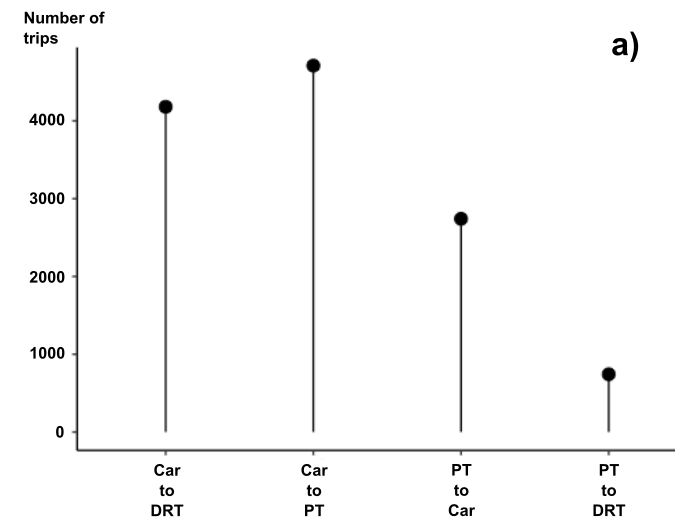
\includegraphics[width=.49\textwidth]{images/switRStrips.png}
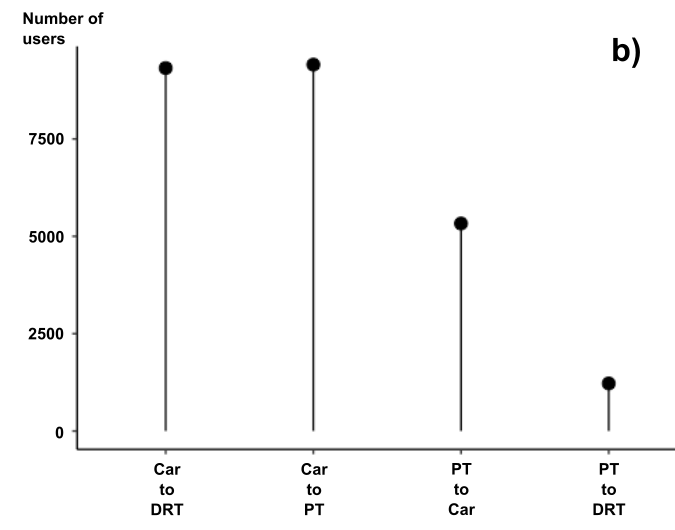
\includegraphics[width=.49\textwidth]{images/switRSusers.png}
  \captionsetup{width=.9\textwidth}
  \caption{Baseline to DRT 300 DtDs 2x Mode Switch of Trips and Users: Figure a) shows the 10\,\% number of trips which agents changed their transport mode from the baseline scenario to the DRT 300 DtDs 2x scenario. It shows the high switching away from car trips and the lower switching from public transport trips. Figure b) shows the 10\,\% number of trips which agents changed their main transport mode from the baseline scenario to the DRT 300 DtDs 2x scenario. Car users are seen to switch in high numbers to public transport and DRT.}
\label{fig:1-2}
\end{figure}

% \textcolor{red}{@andy bitte graphiken größer}
% \begin{figure}[!h]
%   \centering
%   \begin{minipage}[b]{0.4\textwidth}
%   \caption{Baseline to DRT 300 DtDs 2x Mode Switch of Trips.\\
%   The f }
%     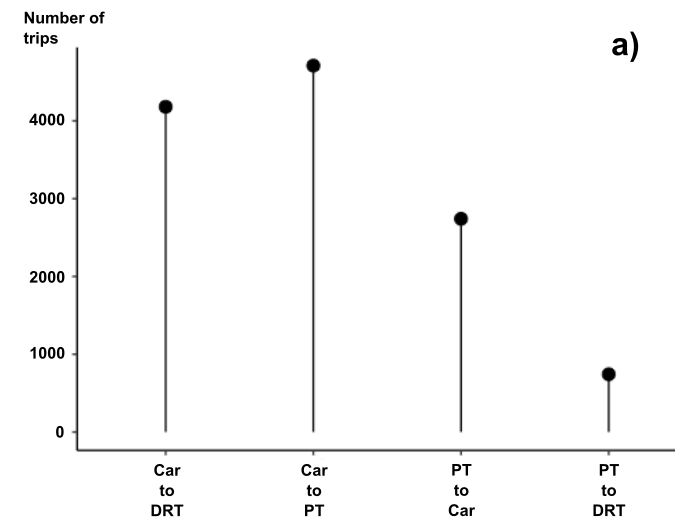
\includegraphics[width=\textwidth]{images/switRStrips.png}
%     \label{fig:1}
%   \end{minipage}
%   \hfill
%   \begin{minipage}[b]{0.4\textwidth}
%   \caption{Baseline to DRT 300 DtDs 2x Mode Switch of Persons\\
%    The figure shows the 10\,\% number of trips which agents changed their main transport mode from the baseline scenario to the DRT 300 DtDs 2x scenario. Car users are seen to switch in high numbers to public transport and DRT.}
%     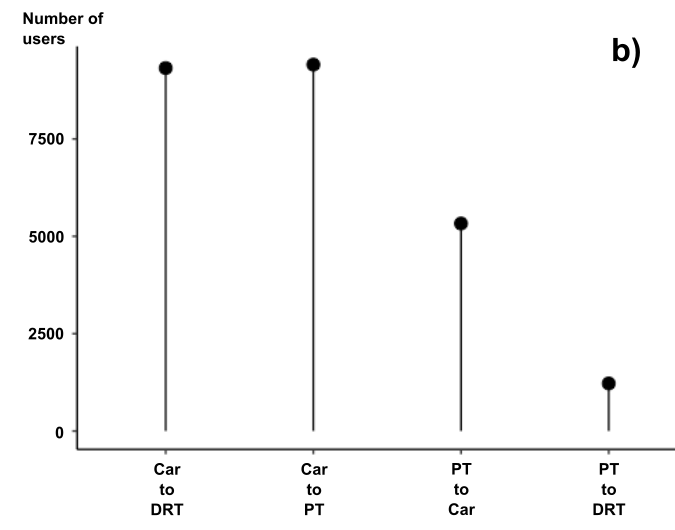
\includegraphics[width=\textwidth]{images/switRSusers.png}
%     \label{fig:2}
%   \end{minipage}
% \end{figure}

Figures \ref{fig:3-4} show the comparison between the baseline and 300 DRT DtDs 2x mode splits. A decrease in public transport use is observed as a trend in both scenarios, while the DRT mode share gained in the 300 DRT DtDs 2x scenario can be seen to capture some of the baseline increase in walking and it leads to a decrease in the car mode share.
The public transport share decrease is slightly larger in the 300 DRT DtDs 2x scenario, but this potentially worrying sign of a small cannibalisation effect is counteracted by the per kilometer mode statistic comparison showing that the kilometers travelled by public transport are significantly changes. The clearer, and more desirable decrease of car kilometers travelled is evident in Figure \ref{fig:5-6}.

Taken together the results may show that there is greater efficiency in the public transport, with less trips but the same distance covered and therefore less stoppages in the system. The issue of cannibalisation in a city such as Cape Town is anyway contested because the public transport system is failing and sub-optimal for city needs, therefore in this case the mode switch away from public transport is not necessarily indicative of negative cannibalisation. The switching data shows that public transport users switch less to DRT than to cars, so replacement is not direct in any case and motivation based policy to decrease car use could maintain public transport use. There is need for further research on integrating public transport and DRT in developing cities such as Cape Town.\\


\begin{figure}[htbp]
\centering
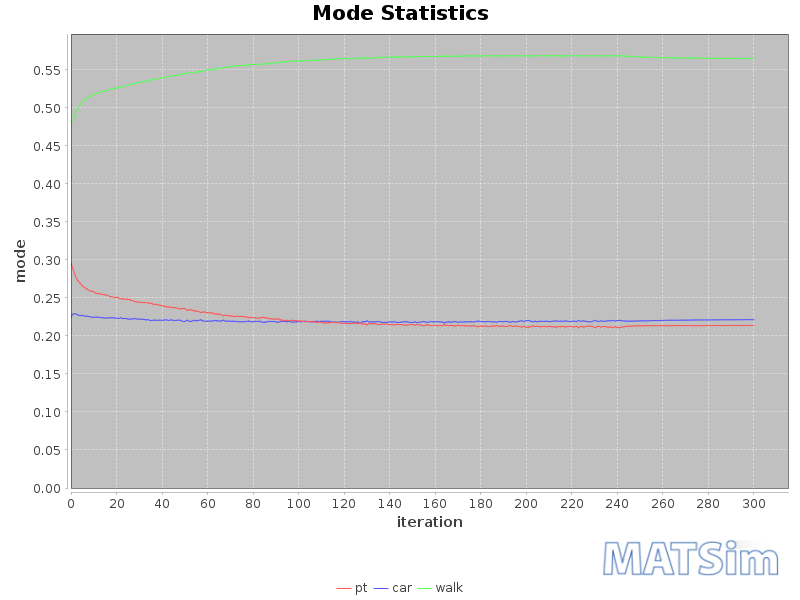
\includegraphics[width=.49\textwidth]{images/baseline_modestats.png}
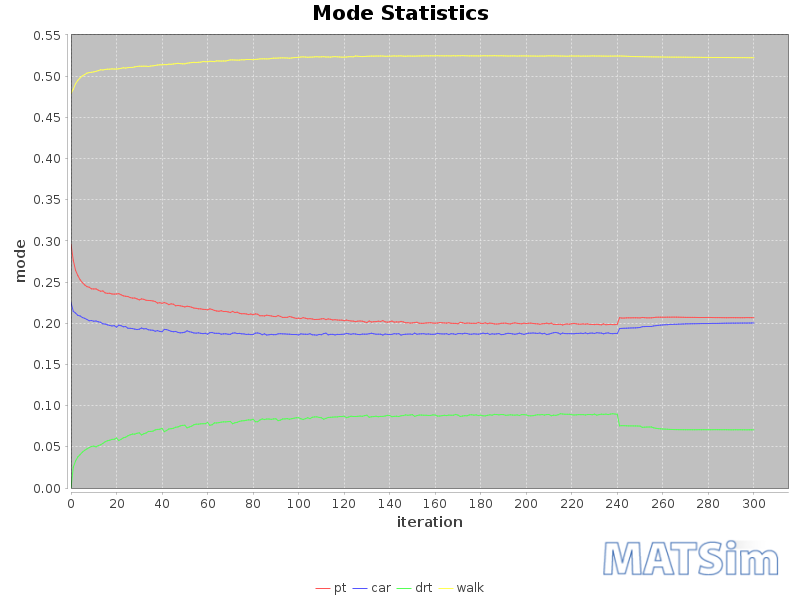
\includegraphics[width=.49\textwidth]{images/modestats.png}
  \captionsetup{width=.9\textwidth}
  \caption{Baseline and DRT 300 DtDs 2x Whole City Mode Statistics: Figure on the left shows how the mode share for public transport (pt), car and walk develops during the 300 iterations of the simulation of the Baseline Scenario for Cape Town. Figure on the right shows how the mode share for public transport (pt), car, walk and DRT develops during the 300 iterations of the simulation of the DRT 300 DtDs 2x Scenario for Cape Town.}
  \label{fig:3-4}
\end{figure}

% \begin{figure}[!h]
%   \centering
%   \begin{minipage}[b]{0.49\textwidth}
%   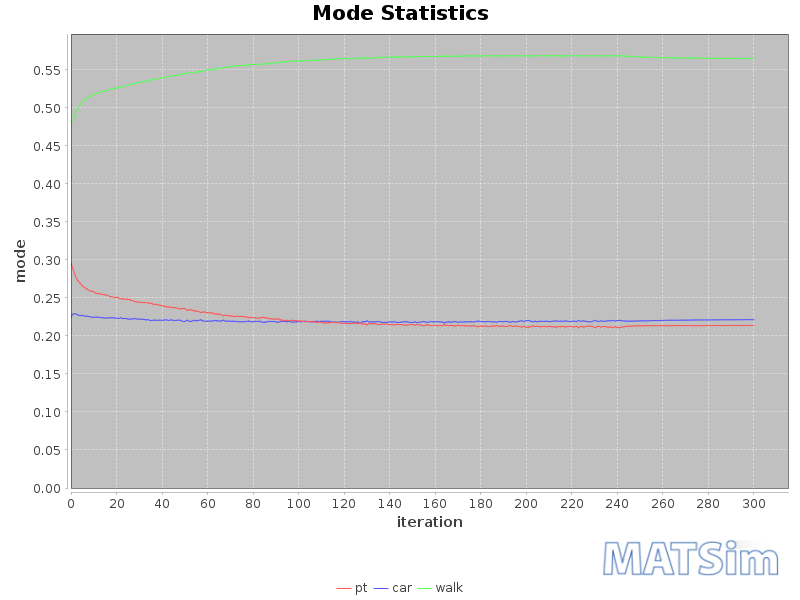
\includegraphics[width=\textwidth]{images/baseline_modestats.png}
%   \caption{Baseline Whole City Mode Statistics\\
%   This figure shows how the mode share for public transport (pt), car and walk develops during the 300 iterations of the simulation of the Baseline Scenario for Cape Town.}
    
%     \label{fig:3}
%   \end{minipage}
%   \hfill
%   \begin{minipage}[b]{0.49\textwidth}
%   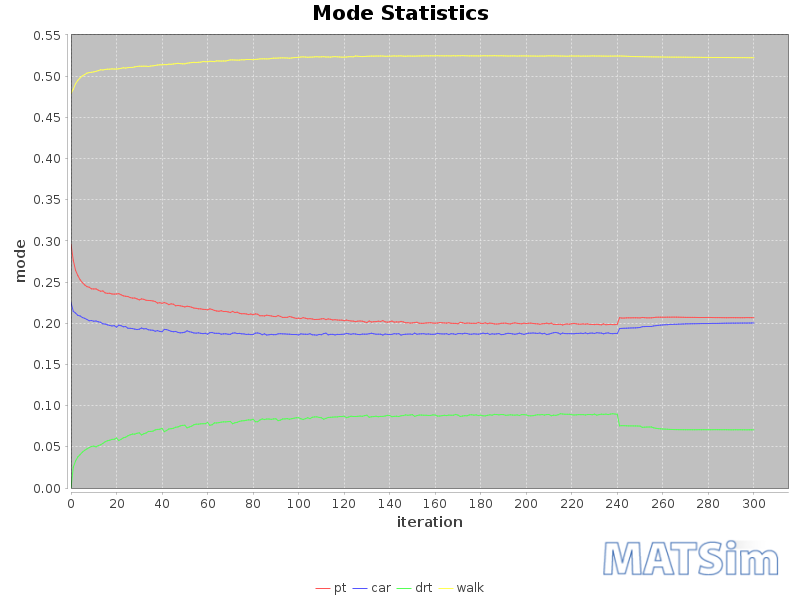
\includegraphics[width=\textwidth]{images/modestats.png}
%   \caption{DRT 300 DtDs 2x Whole City Mode Statistics\\
%   This figure shows how the mode share for public transport (pt), car, walk and DRT develops during the 300 iterations of the simulation of the DRT 300 DtDs 2x Scenario for Cape Town.}
    
%     \label{fig:4}
%   \end{minipage}
% \end{figure}

\begin{figure}[htbp]
\centering
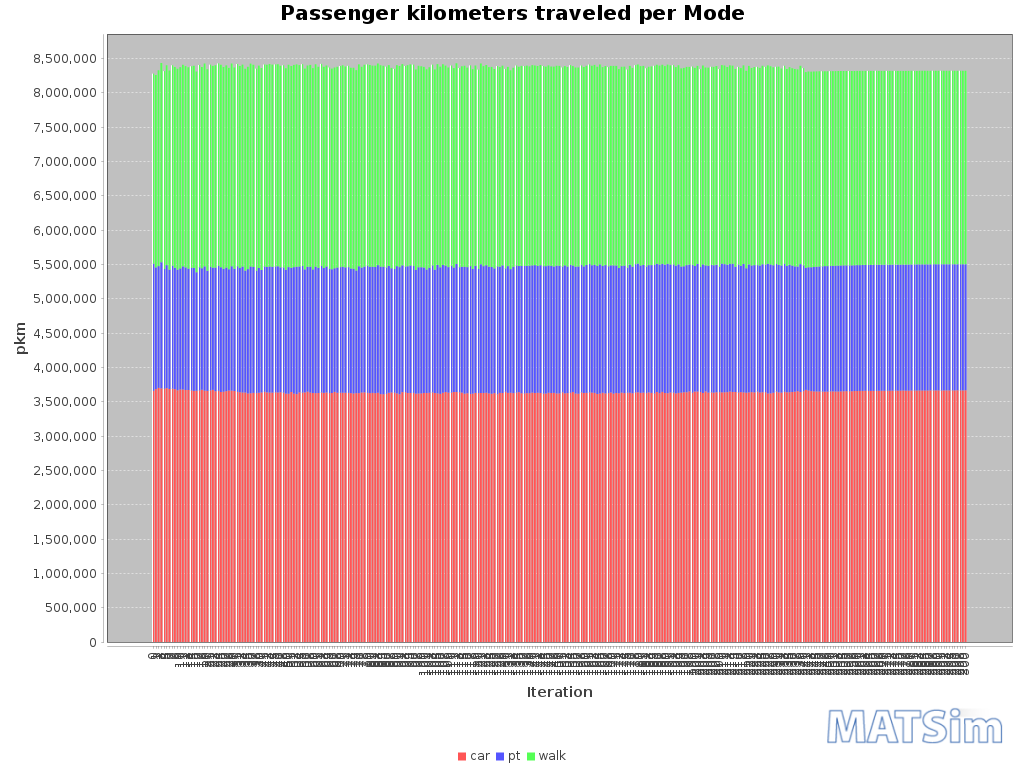
\includegraphics[width=.49\textwidth]{images/baseline_pkm_modestats.png}
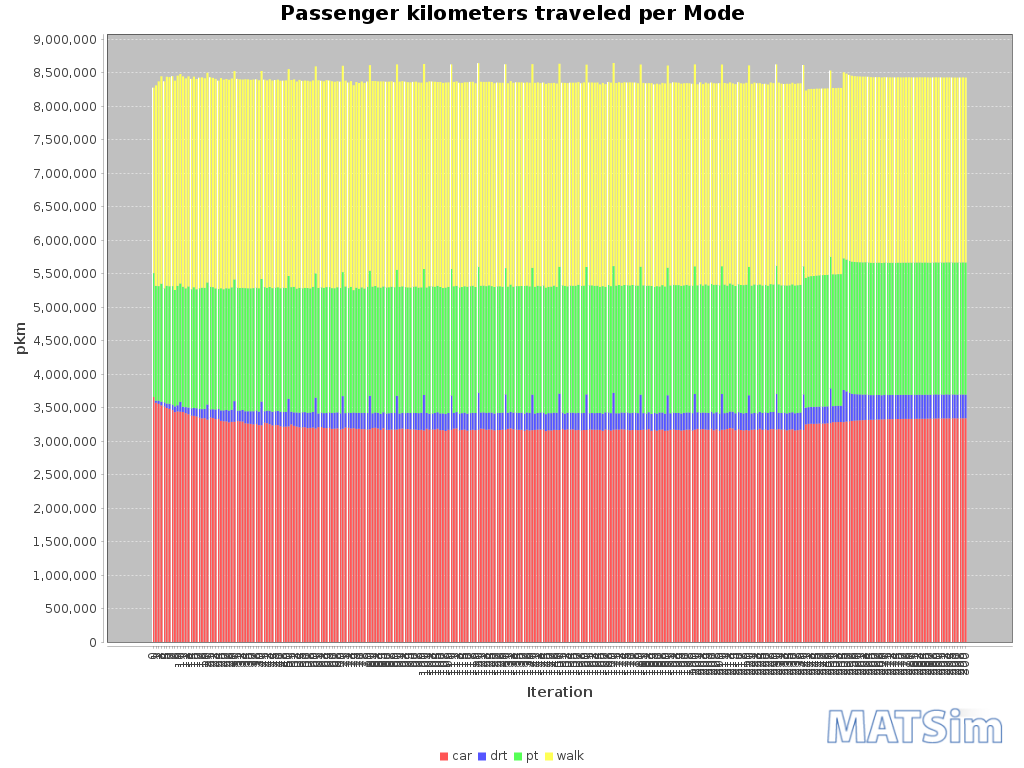
\includegraphics[width=.49\textwidth]{images/pkm_modestats.png}
  \captionsetup{width=.9\textwidth}
  \caption{Baseline and DRT 300 DtDs 2x Whole city per km Mode Statistics: Figure on the left shows how the mode per kilometer for public transport (pt), car and walk develops during the 300 iterations of the simulation of the Baseline Scenario for Cape Town. The car kilometers are clearly the largest, followed by walk and then public transport. Figure on the right shows how the mode per kilometer for public transport (pt), car and walk develops during the 300 iterations of the simulation of the DRT 300 DtDs 2x Scenario for Cape Town. The car kilometers lose some of their dominance from the Baseline as DRT gains a wedge.}
  \label{fig:5-6}
\end{figure}

% \begin{figure}[!h]
%   \centering
%   \begin{minipage}[b]{0.49\textwidth}
%   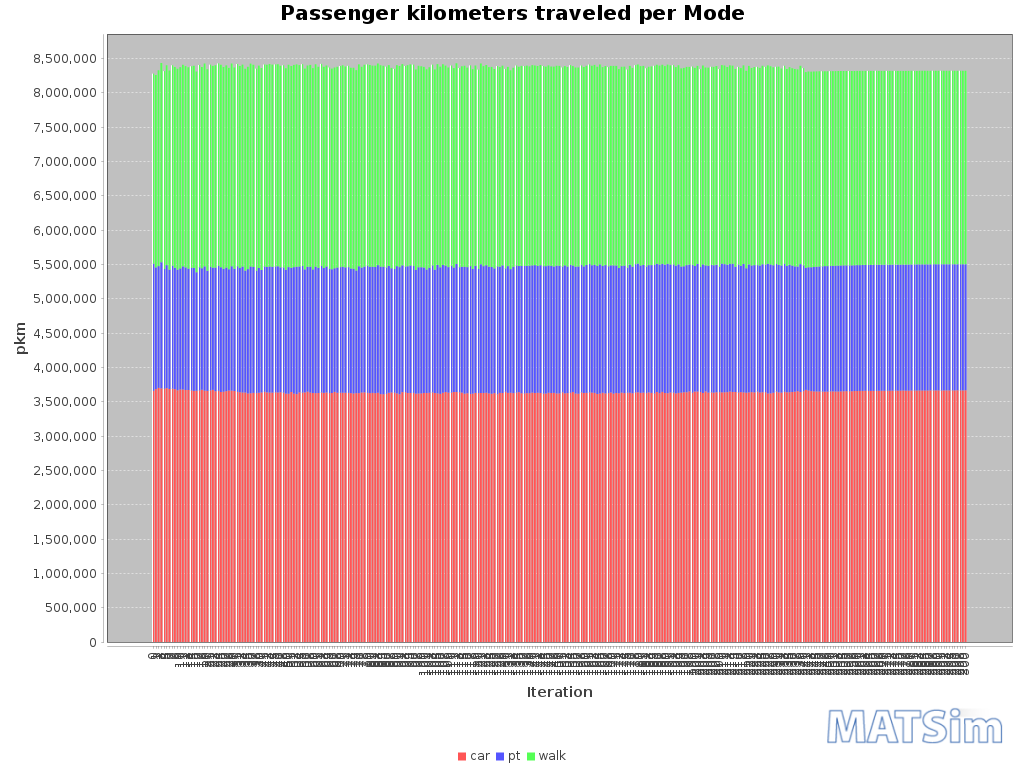
\includegraphics[width=\textwidth]{images/baseline_pkm_modestats.png}
%   \caption{Baseline Whole city per km Mode Statistics\\
%   This figure shows how the mode per kilometer for public transport (pt), car and walk develops during the 300 iterations of the simulation of the Baseline Scenario for Cape Town. The car kilometers are clearly the largest, followed by walk and then public transport.}
    
%     \label{fig:5}
%   \end{minipage}
%   \hfill
%   \begin{minipage}[b]{0.49\textwidth}
%   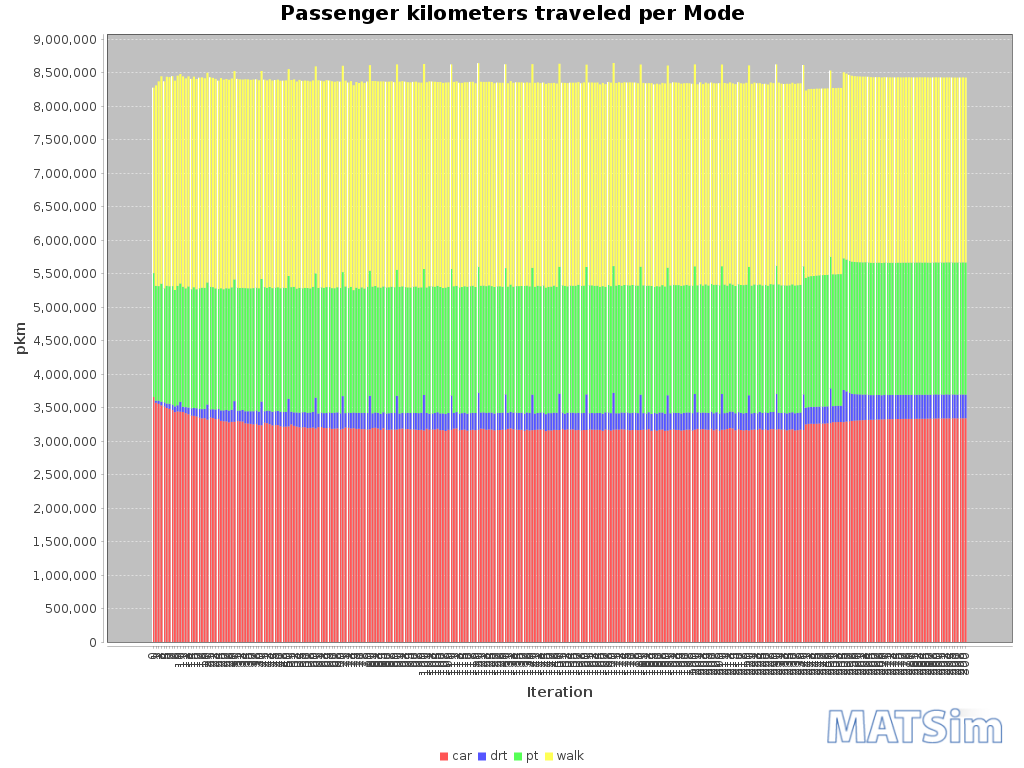
\includegraphics[width=\textwidth]{images/pkm_modestats.png}
%   \caption{DRT 300 DtDs 2x Whole city per km Mode Statistics\\
%    This figure shows how the mode per kilometer for public transport (pt), car and walk develops during the 300 iterations of the simulation of the DRT 300 DtDs 2x Scenario for Cape Town. The car kilometers lose some of their dominance from the Baseline as DRT gains a wedge.}
    
%     \label{fig:6}
%   \end{minipage}
% \end{figure}



Service areas have been known to impact the effect of DRT \citep{kaddoura2020impact, schluter2021impact}. Furthermore since we introduce DRT in particular service areas of a city for greatest impact and efficiency, it is helpful to evaluate the impact within the service areas in comparison the whole city. It is also valuable to understand behaviour of travellers across and within these geographic areas.
The map in Figure \ref{fig:7} shows the groups of connected service areas.
When the results of the 300 DRT DtDs 2x scenario are analysed in the respective service areas which are targeted by DRT, the majority of DRT trips are taken between disconnected groups of service areas. 
The simulation shows that all car use beginning in service areas decreases by 18.6 percent with the introduction of 300 DtDs DRT 2x public transport cost to the baseline. Car trips purely within connected service areas decrease by 28.5 percent. Car use between these service areas decreases by 51 percent. This striking car use decrease between service areas still translates to larger reductions in congestion in service areas however, because the beginnings and ends of these trips converge in the service areas.
\\


Congestion is such a large problem that needs improvement in cities around the world for clear economic and environmental reasons. Our simulations give evidence that introducing DRT would likely improve congestion in many, if not all of these cities.
The results show that in the 300 DtDs 2x cost scenario congestion improves by 14.3 percent for the whole city (Figure \ref{fig:8}). Such decreases could bring major gains to cities, and if stronger policies were to induce the use of larger fleets of DRT paired with sufficient road capacity increases, there is evidence that congestion could even be eradicated in some cases \citep{maciejewski2016congestion}.


\begin{figure}[h]
\centering
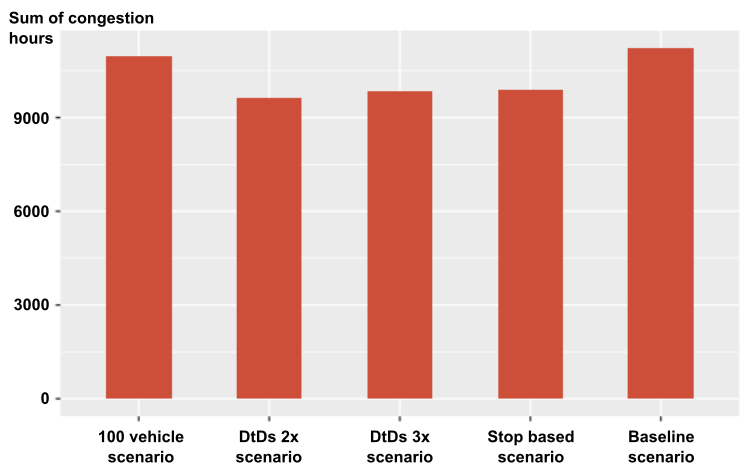
\includegraphics[width=8cm]{images/Cong_WC.png}
\caption{Congestion measurements for the whole city: The sum of congeston hours for various scenarios are compared.}
  \label{fig:8}
 \end{figure}
 
Figures \ref{fig:9-10} show that congestion improvements for the 300 DRT DtDs 2x scenario is greater in service areas than the congestion decrease in the areas excluding the service areas. The 300 vehicle stop based 2x public transport cost (300 DRT SB 2x) scenario, has a different pattern, with congestion inside and outside of the service areas being more on par.\\

\begin{figure}[htbp]
\centering
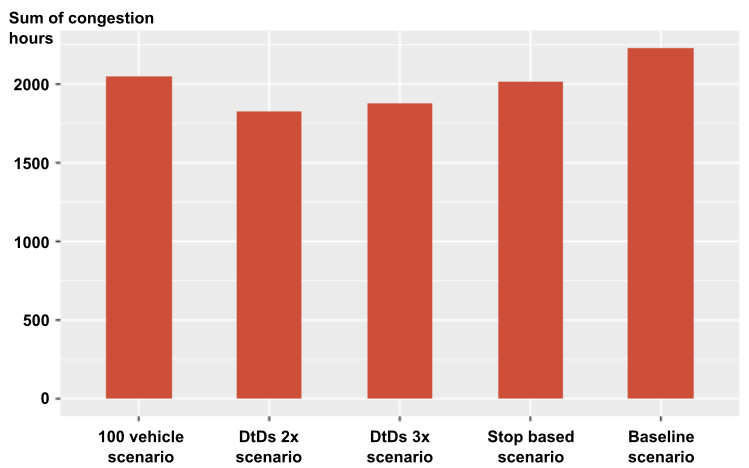
\includegraphics[width=.49\textwidth]{images/S_cong.png}
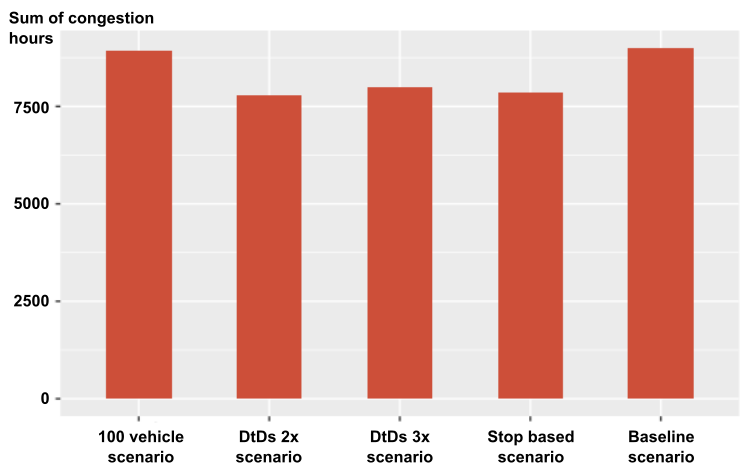
\includegraphics[width=.49\textwidth]{images/XS_cong.png}
  \captionsetup{width=.9\textwidth}
  \caption{Congestion measurements inside and outside service area: Figure on the left compares the sum of congeston hours inside the service areas and figure on the right compares the sum of congeston hours outside the service areas for the various scenarios.}
  \label{fig:9-10}
\end{figure}

% \begin{figure}[h]
%   \centering
%   \begin{minipage}[b]{0.4\textwidth}
%   \caption{Congestion service area\\
%   Here the congestion measurements inside the service areas are compared for the scenarios.}
%     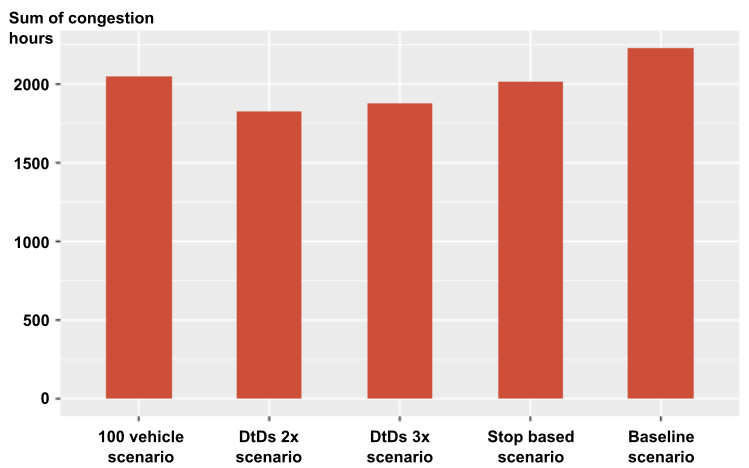
\includegraphics[width=\textwidth]{images/S_cong.png}
%     \label{fig:9}
%   \end{minipage}
%   \hfill
%   \begin{minipage}[b]{0.4\textwidth}
%   \caption{Congestion excluding service area\\
%   Here the congestion measurements in the areas excluding the service areas, are compared for the various scenarios.}
%     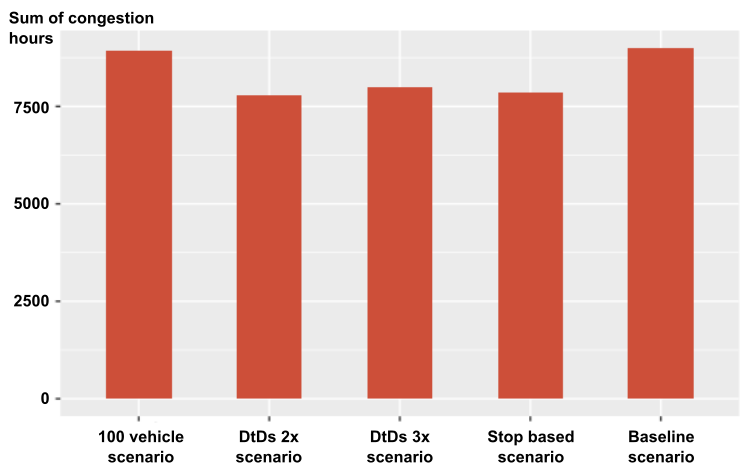
\includegraphics[width=\textwidth]{images/XS_cong.png}
%     \label{fig:10}
%   \end{minipage}
% \end{figure}


\clearpage


The 300 DRT DtDs 2x scenario gave a very good uptake rate, but congestion was slightly less improved than the 300 DRT DtDs 2x scenario especially in service areas. This makes sense as stop based DRT would have higher concentration around stops than random DtDs stops that are more spread around an area. In the 300 DRT SB 2x scenario the average travel time for cars and walking improved, but public transport travel time increased by a large margin. This travel time draw back for the 300 DRT SB 2x scenario, may be outweighed by the accessibility improvements it brings to a city that has under provision of transport to the population. The baseline of an under-provision situation has to be understood as such. This also applies to the travel time increase that occurs in the context of a severely inefficient public transport sector - it may point to the potential to replace current public transport with DRT. The 300 DRT SB 2x scenario is very much like having the current MBT system revamped with ride hailing at taxi ranks. Congestion would likely still be experienced due to the concentration of traffic on main routes between stops, but flow management via technology would improve outcomes significantly. Road capacity increases would even further enhance these efficiency gains. The simulation gives evidence of the potential to improve current MBT systems with technological improvements, while giving heed to possible negative effects on travel time in the city.\\

\begin{figure}[htbp]
\centering
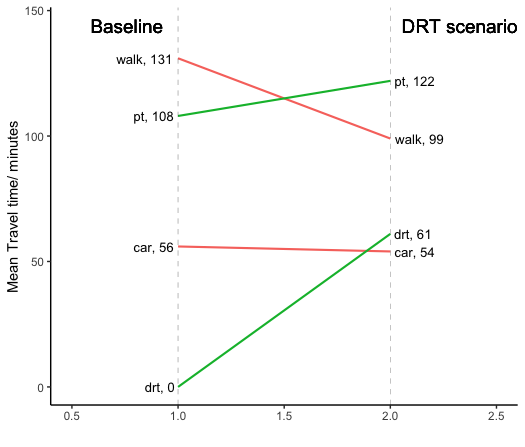
\includegraphics[width=.49\textwidth]{images/DRTstopbasetime.png}
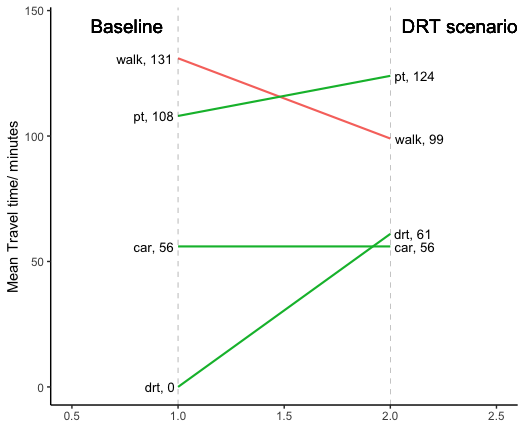
\includegraphics[width=.49\textwidth]{images/DRTrandomstoptime.png}
  \captionsetup{width=.9\textwidth}
  \caption{Travel time for Stop Based DRT and DtDs scenario: On the left figure the average travel time for each mode is compared for the Baseline Scenario and SB DRT 2x Scenario. DRT is set to have 0 travel time in the Baseline where it is not present. Decreased travel time lines are red and increased travel time are green. The average travel time minutes are recorded next to the mode. On the right figure the average travel time for each mode is compared for the Baseline Scenario and DtDs DRT 2x Scenario. DRT is set to have 0 travel time in the Baseline where it is not present. Decreased travel time lines are red and increased travel time are green. The average travel time minutes are recorded next to the mode.}
  \label{fig:11-12}
\end{figure}

% \begin{figure}[!h]
% \centering
%  \begin{minipage}[b]{0.4\textwidth}
% \caption{Travel time for Stop Based DRT scenario\\
% The average travel time for each mode is compared for the Baseline Scenario and SB DRT 2x Scenario. DRT is set to have 0 travel time in the Baseline where it is not present. Decreased travel time lines are red and increased travel time are green. The average travel time minutes are recorded next to the mode.}
% 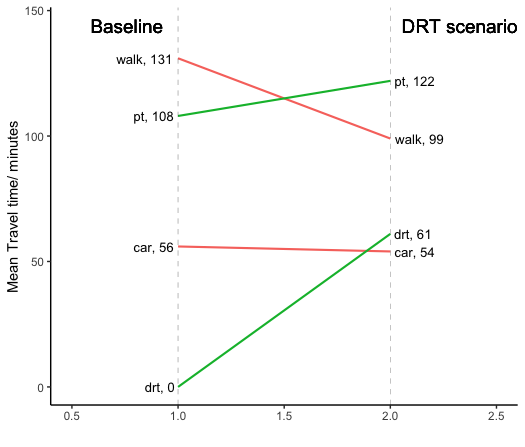
\includegraphics[width=\textwidth]{images/DRTstopbasetime.png}
% \label{fig:11}
%   \end{minipage}
%   \hfill
%   \begin{minipage}[b]{0.4\textwidth}
% \caption{Travel time for DtDs scenario,\textcolor{red}{sind die notwendig}\\
% The average travel time for each mode is compared for the Baseline Scenario and DtDs DRT 2x Scenario. DRT is set to have 0 travel time in the Baseline where it is not present. Decreased travel time lines are red and increased travel time are green. The average travel time minutes are recorded next to the mode.}
% 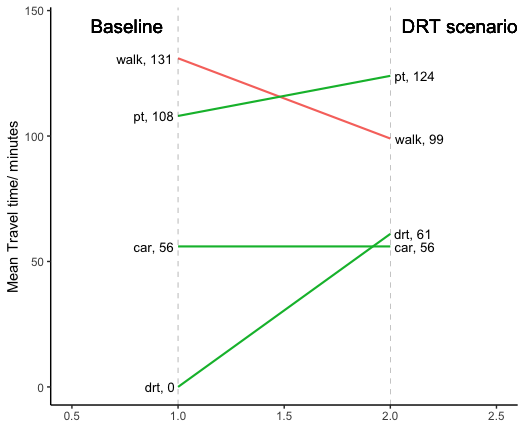
\includegraphics[width=\textwidth]{images/DRTrandomstoptime.png}
% \label{fig:12}
%   \end{minipage}
% \end{figure}


Travel time is closely related to congestion, as it is often used to measure congestion. Travel time and congestion are especially linked for travel modes such as car and DRT, and for public transport that includes buses, and MBT's in the case of Cape Town. The simulation data for the 300 DRT DtDs 2x scenario shows that average car travel time remains the same when DRT is introduced (Figure \ref{fig:11-12}). These time effects on the whole city are not impressive, but dis-aggregating the travel time to within connected service area travel, and between service area average car travel time the strong effect becomes clear. While within service area average travel time for cars has a one minute increase, between service areas car travel time decrease by 26 percent. Aligning with the findings of decreased car use between service areas and most DRT trips between service areas, this translates to significant decreases in the travel time between respective groups of service areas. The saving of time brought by introducing just a small fleet of DRT is remarkable, and points to the efficiency gains of the intervention. There is however greater DRT average travel time than average car travel time (shown in Figure \ref{fig:9-10}) and this may mean that policy would need to incentivise travellers away from car use toward DRT to get the overall system efficiency gain of introducing DRT.\\



Our modelling of the 300 DRT DtDs 2x scenario, gave insight into some interesting outcomes.
Total trips taken decreased by 0.04 percent. Since public transport and paratransport in the Cape Town context include buses and MBT's which contribute to congestion without the gain of flow optimisation that app based DRT technology allows, the relative share of DRT replacing cars and even some public transport trips, leads to better total travel time and congestion outcomes even though it adds greater trip numbers than the cars it eliminates.\\

Environmental concerns must be evaluated when bringing changes to a transport system.
The emissions data from our simulations show that the scenarios with low uptake such as the 3x price or 100 vehicle scenarios bring improvements to emissions (Figure \ref{fig:15}, Figure \ref{fig:16}) alongside their small improvements to congestion (Figure 8). The 2x price scenario which has greater congestion impact brings no improvement to emissions, and this highlights the trade off between these outcomes when traditional fuels are used. The potential to use electric DRT vehicles can change this outcome. Evaluating the traditional fuel scenario carbon dioxide pollution changes from the baseline are negligent for the 300 DRT DtDs scenarios (Figure \ref{fig:15}). The Nitrogen Oxide impact is not so positive when evaluating the 300 DRT DtDs scenarios, as the baseline or 100 DRT vehicle scenario show lower emissions (Figure \ref{fig:16}). The trade off between much needed economic efficiency in developing countries and incremental environmental damage increases the impetus to look into using electric vehicles of DRT fleets, which many speed up electrification compared to private car uptake. \\

A result that is relevant for cities where public transport is low quality or requires high waiting time is that DRT waiting times are much lower than public transport waiting times. DRT gives a viable option which can improve accessibility. It may be useful for miscellaneous and one-off travel needs for low income users such as job searches and interviews that are not modelled. DRT can improve waiting times for public transport especially if it is integrated into a public transport system. Integrating DRT into public transport systems is being explored in new research and applications \citep{byala2021redesigning, Loubser, becker2020assessing}\\



\begin{table}[!h]
\centering
\begin{tabular}{|l|l|l|}
\hline
Scenario            & Public Transport wait time & DRT wait time \\ \hline
Baseline &44.29 & -                    \\ \hline
300 DRT DtDs 2x              & 46.22 & 10.48                       \\ \hline
300 DRT SB 2x              & 45.47 & 7.23                   \\ \hline
\end{tabular}

\caption{Wait time in minutes}
\label{Wait times}
\end{table}


Our results show that a small amount of DRT vehicles added into the city causes large impacts on the amount of cars on the road and congestion. Figure 13 and Figure 14 compare these as percentages for the whole city and for the service areas. The bars represent; the amount of DRT vehicles in an area compared to the total amount of private cars, and the ensuing decrease in cars as a proportion of the total, and the congestion decrease experienced in the area. \\

\begin{figure}[htbp]
\centering
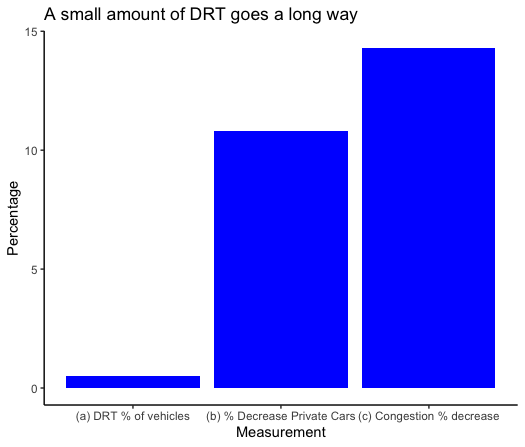
\includegraphics[width=.49\textwidth]{images/carwholecity.png}
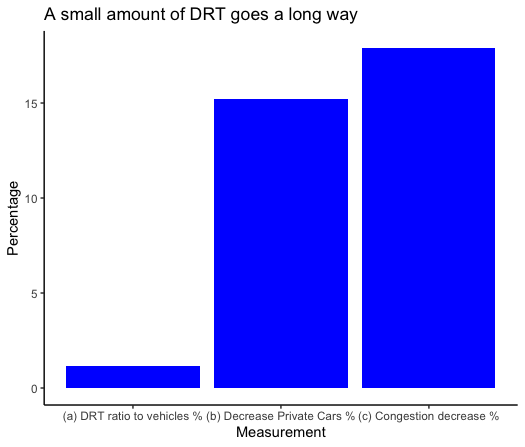
\includegraphics[width=.49\textwidth]{images/cars_servarea.png}
  \captionsetup{width=.9\textwidth}
  \caption{DRT impact on the Whole City and Service Area DRT scenario: On the left figure the bar plot shows the impact of DRT by comparing the percentage of vehicles on the city's roads that DRT represents, to the percentage of private cars decreasing from the Baseline to DtDs 2x scenario, and to the percentage decrease in congestion experienced in the city. On the right figure the bar plot shows the impact of DRT in the service areas by comparing the percentage of vehicles in the service areas that DRT represents, to the percentage of private cars used in the service areas decreasing from the Baseline to DtDs 2x scenario, and to the percentage decrease in congestion experienced in the service areas.}
  \label{fig:13-14}
\end{figure}

% \begin{figure}[!h]
%   \centering
%   \begin{minipage}[b]{0.4\textwidth}
%   \caption{Whole City DRT impact\\
%   This bar plot shows the impact of DRT by comparing the percentage of vehicles on the city's roads that DRT represents, to the percentage of private cars decreasing from the Baseline to DtDs 2x scenario, and to the percentage decrease in congestion experienced in the city.}
%     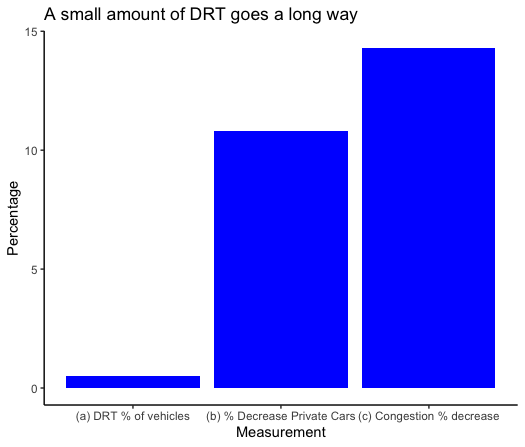
\includegraphics[width=\textwidth]{images/carwholecity.png}
%     \label{fig:13}
%   \end{minipage}
%   \hfill
%   \begin{minipage}[b]{0.4\textwidth}
%   \caption{Service Area DRT impact\\
%    This bar plot shows the impact of DRT in the service areas by comparing the percentage of vehicles in the service areas that DRT represents, to the percentage of private cars used in the service areas decreasing from the Baseline to DtDs 2x scenario, and to the percentage decrease in congestion experienced in the service areas.}
%     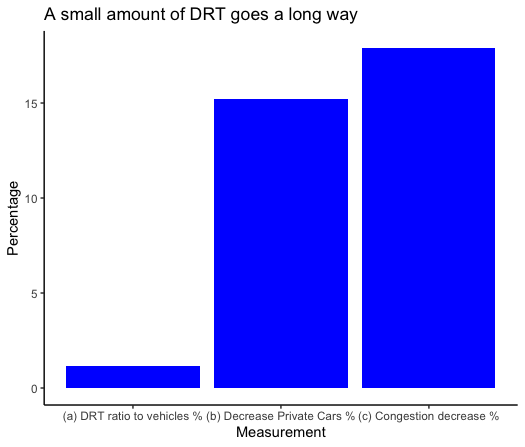
\includegraphics[width=\textwidth]{images/cars_servarea.png}
%     \label{fig:14}
%   \end{minipage}
% \end{figure}


 Overall the findings point toward a positive contribution of DRT to congestion in developing country cities when introduced in affluent service areas. There is a greater decrease of cars and travel time out of service areas which shows the positive externalities on the traffic system that a DRT program targeting the affluent areas can have. 
 The potential for automated and electric DRT still remains and can be implemented on a model of fuel based driver DRT that is implemented to improve traffic outcomes.\\
 

\section*{Conclusion}
%\textcolor{red}{Estelle today}\\
This paper began with the problem of congestion and the research question of investigating the impact of DRT on city congestion in Capetown. A brief review of literature on DRT and its modelling with MATsim and related issues, gave background for the paper. We hypothesised that DRT would be a beneficial addition to transport systems in developing cities like Cape Town. In the context of the Cape Town transport system, simulations were used to show that introducing medium sized fleets of DRT vehicles at double the price of public transport improves congestion outcomes significantly. Various scenarios were explored to find the optimal fleet size and pricing within the modelling constraints. The improvements are seen to impact mode share and switching, and waiting and travelling time, while having negligent effects on emissions if electric vehicles are not used. 


\pagebreak

\bibliographystyle{apalike}
\bibliography{ref}


\appendix
\section*{Appendix}

\begin{figure}[!h]
\centering
\caption{Co2 Emissions}
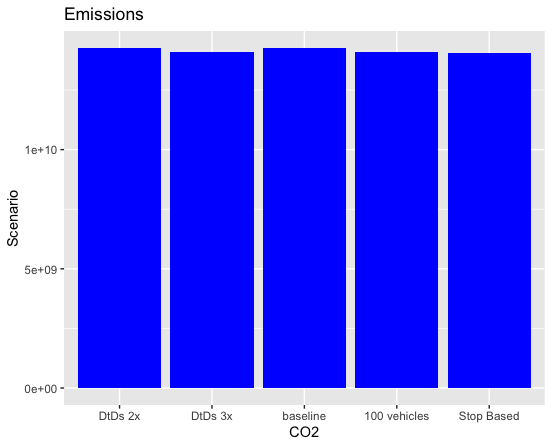
\includegraphics[width=10cm]{images/Co2_new.png}
  \label{fig:15}
\end{figure}


\begin{figure}[!h]
\centering
\caption{NOx Emissions}
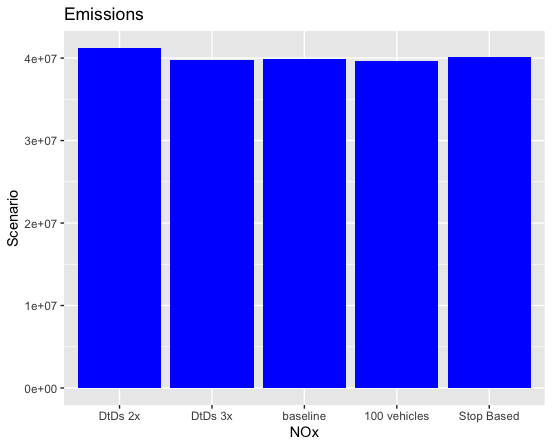
\includegraphics[width=10cm]{images/Nox_new.png}
  \label{fig:16}
\end{figure}


The basis of an agent-based MATSim simulation is a synthetic population of the case study area. For Switzerland, a range of rich
data sources are available that make it possible to set up such a population with detailed socio-demographic and behavioral attributes.
In the following, the process will be described in brief. A more detailed description of the Swiss data sets and how they have been
processed can be found in (H¨orl, 2020). Furthermore, (H¨orl and Balac, 2020) describes the methodology in detail for the case of Paris
and ˆIle-de-France. There, unlike Switzerland, all necessary data sets are publicly and openly available to replicate the process.
Initially, the synthetic Swiss population is based on the STATPOP data set, which is a comprehensive census of Switzerland,
including attributes like age and gender of all residents, but - most notably - also location by coordinate of each household. Persons and
households from this data set are used directly as a basis of the Swiss synthetic population. Afterward, work or educational locations for
each synthetic person are added. For that, the Structural Survey is used, which, unlike the registration-based census data, is a detailed
household survey conducted for around 3% of the Swiss population each year. From this data set, an origin–destination matrix between
home and work/education municipalities in Switzerland can be derived, then used to proportionately sample destination zones for
each agent, based on their home zone. In the third step, the national Mobility and Transport Microcensus is employed: a classical
household travel survey providing full day activity patterns for around 60,000 respondents. We use a statistical matching procedure to
sample and attach activity chains to the synthetic persons, based on socio-demographic attributes. This way, activity patterns
correlating with certain age groups or gender are assigned according to the population. These activity chains contain activity types,
activity durations and connecting modes of transport as reported in the survey data. As departure and arrival times are rounded
strongly (in five minute intervals) as is the case in many surveys, activity chains (including all departure and arrival times) are shifted
by a random offset of +/- 30 min for each person to avoid having unrealistically many people departing at the same time at one
location, which would, in turn, affect the traffic dynamics in the simulation negatively. Finally, specific work and education locations
are sampled, based on the destination zones of the agents, from STATENT, the national enterprise census, which lists all facilities in
Switzerland by coordinate. Further, secondary activities in the agents’ plans (such as shopping or leisure), are assigned to discrete
facilities using a specifically-designed algorithm for secondary location assignment (H¨orl and Axhausen, 2020). To complete the
simulation data, an exhaustive digital public transit schedule for Switzerland is integrated into the simulation and the road network is
extracted from OpenStreetMap, including all roads from motorways to residential roads. In total, this process yields a synthetic
representation of Switzerland that reproduces the daily mobility needs of the population and available infrastructure.


Note that MATSim, in
principle, is also able to consider departure time choices or even location choice through its co-evolutionary algorithm, which is a
different process of decision-making not used here; our goal was to directly integrate a discrete choice model into MATSim. Unlike the
standard approach, it inherently contains consistent information about the trade-offs people make between choice dimensions when
faced with the automated mobility option. The standard co-evolutionary algorithm would only allow us to perform sensitivity analyses
on the relatively unspecific attractively level of the new transport mode.Due to the complexity of the simulation, the dense network and the large number of agents, we restrict simulations to 10% samples
of the population, with road capacities being scaled down accordingly


We use a statistical matching procedure to sample and attachactivity chains to the synthetic persons, based on socio-demographic attributes. This way, activity patternscorrelating with certain age groups or gender are assigned according to the population. These activity chainscontain activity types, activity durations and connecting modes of transport as reported in the survey da

For the simulation of mobility behaviour we utilise the multi-agent transport simulation framework MATSim version 14.0 \citep{Horni.2016}. A synthetic scenario of Cape Town with a population sample size of 10\,\% is employed for the study. We derive the synthetic population from South African Census Data 2011 \citep{census2011}, the 10\% Public Use Sample \citep{census2011public10pct} and the Minnesota Population Center Integrated Public Use Microdata Series \citep{mpc2020}. For the population synthesis process we employ a mlti-level iterative proportional fitting methodology \citep{joubert2014mipf}. Furthermore, we utilize data from National Household Travel Survey 2013 \citep{nhts2013} and the Time Use Survey 2010 \citep{tus2013} to assign individual mobility behaviour to the synthetic agents.  \\


On the supply side we employ network and infrastructure data from OpenStreetMap (OSM) \citep{osm}. The network links are downscaled according to the population sample in terms of flow and storage capacities. Furthermore, the individual OSM ids of the dataset are extracted and categorised into different activities such as "shopping" or "leisure". In addition, we use GTFS datasets from the main public transport providers in Cape Town from 2018 to model public transport \citep{transifeeds}. The capacities of the vehicles are also downscaled according to the population sample, as the adjustment of the vehicle size to the downscaled network leads to a distortion of the passenger flows. To avoid further distortions in the timetables of the vehicles by the other network participants and for reasons of simplification, the vehicles of Golden Arrow Bus Services (GABS), Metrorail Western Cape, MyCiTi Cape Town Integrated Rapid Transit (IRT) system and UCT campus shuttle buses (Jammie) operate on a pseudo-network with direct aerial lines between stops and with adjusted speed limits on each route to match the timetable. For the modelling of informal public transport in the form of minibus taxis, the use of a pseudo-network is omitted due to the fact that the number of minibus taxis is significantly higher than in the case of formal public transport which leads to feedback effects in the traffic flow. To represent these effects in the overall traffic in Cape Town the Minibus Taxis travel together with the other individual traffic on the OSM motor roads.\\


Again, using the OSM data, the modelled infrastructure and the socio-demographic characteristics of the agents such as age, gender and employment status, a gravity model is used to create a path-destination matrix and assign it to the agents. The resulting base population then goes through several calibration steps, calibrating towards NHTS averages and Cape Town Vehicle Detection System (VDS) traffic flow data on major roads from 2018. The calibration target is set at an average deviation from real data of less than 20\% error for car traffic and less than 50\% for formal and informal public transport.\\


\end{document}
